% vim: set wrap


\section{Symmetry}


There are 37 cells on a size 4 board, but from the starting position only 6 of them are distinct. The rest are equivalent by symmetry or rotation, since the board has 6-fold rotational symmetry and 2-fold mirror symmetries. By storing a zobrist hash for each of the 12 possible board orientations and taking the minimum value as the representative hash, symmetries can be found and ignored. Note that this does not find transpositions, only 1 ply symmetries. As stones are placed, the number of possible symmetries decreases dramatically. Symmetrical moves are ignored for the first five ply at node expansion. After 5 ply, the cost of calculating the extra hash values and finding the unique moves becomes too expensive and so symmetry detection is turned off for all later moves.


\section{Monte Carlo Tree Search Solving}

Section \ref{sec:proofbackups} showed that MCTS is capable of solving non-trivial positions in reasonable time. This section will show a couple improvements to MCTS that make it better suited to solving harder positions.

\subsection{Multi-threading}

Solving a position usually takes significantly more effort than merely being fairly sure of the right move. Therefore it is important to use as much computation power as possible. On todays multi-core machines, this means multi-threading.

Writing fast and thread safe code is a challenge. The player threads are spawned in a thread pool that follow a simple state machine. State updates are done using atomic compare and swap (CAS) machine instructions to ensure all state transitions are race-free, and to avoid locks and their contention. Barriers are used to pass control between the control thread and the player threads, and to synchronize the player threads for garbage collection which is a single threaded procedure.

All updates to values in the MCTS tree are also updated with atomic instructions. Updating experience or rave values are done using atomic increment instructions. Adding children is done with CAS to update the value of the children pointer. If multiple threads attempt to create the same set of children only one will succeed and the other will instead do a simulation from the parent node. If multiple threads are backing up the outcome of a node in the tree, and the value has changed unexpectedly, the backup is retried to ensure correctness.

To encourage the threads to explore different parts of the tree, virtual losses are added as each thread descends the tree. These are added atomically as well.

Contention between threads must be minimized to maximize speed. One early source of contention was generating random numbers for the simulations. The rand() function in C++ is very fast in a single threaded environment, but has a lock that limits thread scaling. To avoid this the MTRand library was modified to not use global state and then one instance is used per thread. By having the structure local to each thread no lock is needed and memory contention is minimized.

Pondering, thinking during the opponents time, is a simple way of improving the strength of a player, and is quite easy given the thread pool described above, but it also makes long running solving attempts convenient. The control thread continues to respond to commands while pondering, making it possible to query the state of the player to see the status of the solving attempt. This was instrumental in figuring out why some of the openings were taking so long.


\subsection{Garbage collection}\label{sec:gc}

When solving a non-trivial position, the size of the tree is likely to be bigger than physical memory. For very hard problems it may be several orders of magnitude bigger than physical memory. Large portions of the tree is likely to be irrelevant at any given time however, so can be thrown away when the available memory is filled. If it is needed later, it can be recomputed. Various criteria for which part of the tree can be thrown away are possible, but the one used here is to discard the children of nodes that have fewer than a certain number of simulations. This number of simulations is increased for the next garbage collection if less than half of the memory is freed, and decreased if more than half the memory is freed.


\subsection{Memory Management}

Garbage collection as described in Section \ref{sec:gc} frees enough memory to continue, but malloc/free tend to fragment memory over time, leaving pockets of permanently unusable memory, decreasing the usable available memory. In a player this fragmentation is unlikely to make a difference as the run time is short enough that the fragmentation is a small fraction of total memory. In a long running solver fragmentation could use up to half of the available memory, likely leading to a severe performance hit as the system swaps memory to disk. To avoid this, a compacting tree was implemented. It periodically rearranges the nodes in the tree to avoid fragmentation, while allowing the full memory to be used. This also allows a very fast bump allocation strategy to be used.


\subsection{Early Draw Detection}

Simply checking the outcome at node expansion, and backing up wins, losses and draws as described in Section \ref{sec:proofbackups} above is enough to solve any position, given sufficient time. Certain interesting positions in Havannah lead to many draws, and can take prohibitively long to solve without more advanced draw detection. Figure \ref{fig:drawnowin} shows a board where no wins are possible after move 30 even if both players cooperate. Without draw detection this will take $7!$ simulations to enumerate and prove. In a player this isn't important, since its win ratio approaches the correct value of a draw quickly, but this is not rigorous enough for a solver.

The three win conditions need to be checked to see if any wins of that type are possible. Fork and bridge wins can be detected with the heuristic described in Section \ref{sec:distwin}. Start a flood fill from each corner and edge for each player. If none of the empty cells can reach three edges or two corners for a player, then that player can not form a fork or bridge. One player being unable to form a bridge or fork does not preclude the other player from doing so.

Potential rings can be detected by checking for encirclability. A group of stones that connects to an edge or corner cannot be encircled by the opponent. Any cell that is next to a group that connects to an edge or corner also cannot be encircled by the other player. If no cells can be encircled, then no rings are possible.

If no forks, bridges or rings are possible for a player, then that player cannot win, and so should force a draw if possible. If both players are forcing a draw, then it is a proven draw.

More advanced techniques of draw detection based on virtual connections could detect draws much earlier, possibly as early as move 20 in Figure \ref{fig:drawproven}, but these techniques have not been explored. The speedup from the techniques described here may not be as large as $7!$ for all boards, but it is still at least an order of magnitude for most early draws.


\section{Solution to Havannah Sizes 2, 3 and 4}

The solutions to board sizes 2, 3 and 4 are shown in this section and in Figure \ref{fig:solutionboard} in particular. The colour of the piece represents the player that will win the game if the white makes his first move on that cell. The subsections describe the proofs in more detail.

\begin{figure}[tb]
\centering
	\subfloat[]{\label{fig:soln2}
		\begin{HavannahBoard}[board size=2,coordinate style=classical,show coordinates=false]
		\HStoneGroup[color=white]{a1,a2,b1,b3,c2,c3}
		\HStoneGroup[color=black]{b2}
		\end{HavannahBoard}
	}
	\subfloat[]{\label{fig:soln3}
		\begin{HavannahBoard}[board size=3,coordinate style=classical,show coordinates=false]
		\HStoneGroup[color=white]{a1,a3,c1,c5,e3,e5}
		\HStoneGroup[color=black]{a2,b1,b2,b3,b4,c2,c3,c4,d2,d3,d4,d5,e4}
		\end{HavannahBoard}
	}
	\subfloat[]{\label{fig:soln4}
		\begin{HavannahBoard}[board size=4,coordinate style=classical,show coordinates=false]
		\HStoneGroup[color=white]{a1,a2,a3,a4,b1,b2,b3,b4,b5,c1,c2,c3,c4,c5,c6,d1,d2,d3,d4,d5,d6,d7,e2,e3,e4,e5,e6,e7,f3,f4,f5,f6,f7,g4,g5,g6,g7}
		\end{HavannahBoard}
	}
\caption{(a) Solution to size 2 (b) Solution to size 3 (c) Solution to size 4}
\label{fig:solutionboard}
\end{figure}


\subsection{Size 2 Proof}

Size 2 Havannah is a trivial game, with the solution shown in Figure \ref{fig:soln2}. It has 6 corners, no edges and a center. The corner opening is a win, since no reply will block both the neighbouring corners. The center is a loss, since it doesn't help any win, nor block a corner win for the other player.

\subsection{Size 3 Proof}

\begin{figure}
\centering
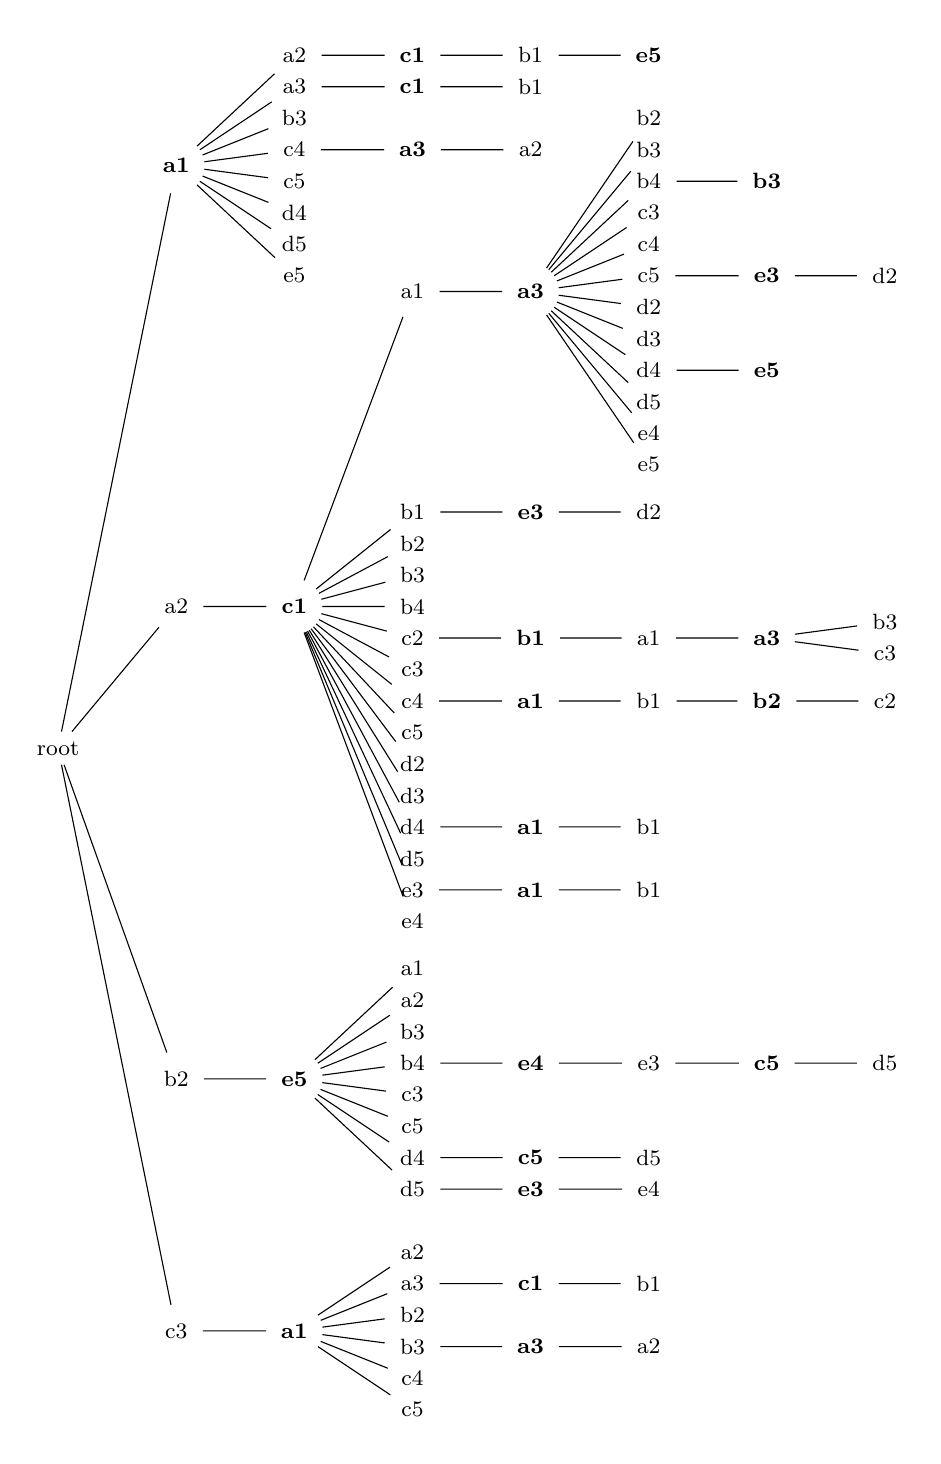
\begin{tikzpicture}[
	font=\footnotesize,
	grow'=right,
	level distance=15mm,
	level 1/.style={sibling distance=4mm},
	level 2/.style={sibling distance=4mm},
	level 3/.style={sibling distance=4mm},
	ww/.style={circle,font=\footnotesize\bfseries},
	wb/.style={circle},
	bw/.style={circle},
	bb/.style={circle,font=\footnotesize\bfseries},
	]
\node {root}
	child { node [ww] {a1}
		child { node [bw] {a2}
			child { node [ww] {c1}
				child { node [bw] {b1}
					child { node [ww] {e5} }
				}
			}
		}
		child { node [bw] {a3}
			child { node [ww] {c1}
				child { node [bw] {b1} }
			}
		}
		child { node [bw] {b3} }
		child { node [bw] {c4}
			child { node [ww] {a3}
				child { node [bw] {a2} }
			}
		}
		child { node [bw] {c5} }
		child { node [bw] {d4} }
		child { node [bw] {d5} }
		child { node [bw] {e5} }
	}
	child [missing] foreach \a in {1,...,13} { }
	child { node [wb] {a2}
		child { node [bb] {c1}
			child { node [wb] {a1}
				child { node [bb] {a3}
					child { node [wb] {b2} }
					child { node [wb] {b3} }
					child { node [wb] {b4}
						child { node [bb] {b3} }
					}
					child { node [wb] {c3} }
					child { node [wb] {c4} }
					child { node [wb] {c5}
						child { node [bb] {e3}
							child { node [wb] {d2} }
						}
					}
					child { node [wb] {d2} }
					child { node [wb] {d3} }
					child { node [wb] {d4}
						child { node [bb] {e5} }
					}
					child { node [wb] {d5} }
					child { node [wb] {e4} }
					child { node [wb] {e5} }
				}
			}
			child [missing] foreach \a in {1,...,6} { }
			child { node [wb] {b1}
				child { node [bb] {e3}
					child { node [wb] {d2} }
				}
			}
			child { node [wb] {b2} }
			child { node [wb] {b3} }
			child { node [wb] {b4} }
			child { node [wb] {c2}
				child { node [bb] {b1}
					child { node [wb] {a1}
						child { node [bb] {a3}
							child { node [wb] {b3} }
							child { node [wb] {c3} }
						}
					}
				}
			}
			child { node [wb] {c3} }
			child { node [wb] {c4}
				child { node [bb] {a1}
					child { node [wb] {b1}
						child { node [bb] {b2}
							child { node [wb] {c2} }
						}
					}
				}
			}
			child { node [wb] {c5} }
			child { node [wb] {d2} }
			child { node [wb] {d3} }
			child { node [wb] {d4}
				child { node [bb] {a1}
					child { node [wb] {b1} }
				}
			}
			child { node [wb] {d5} }
			child { node [wb] {e3}
				child { node [bb] {a1}
					child { node [wb] {b1} }
				}
			}
			child { node [wb] {e4} }
		}
	}
	child [missing] foreach \a in {1,...,14} { }
	child { node [wb] {b2}
		child { node [bb] {e5}
			child { node [wb] {a1} }
			child { node [wb] {a2} }
			child { node [wb] {b3} }
			child { node [wb] {b4}
				child { node [bb] {e4}
					child { node [wb] {e3}
						child { node [bb] {c5}
							child { node [wb] {d5} }
						}
					}
				}
			}
			child { node [wb] {c3} }
			child { node [wb] {c5} }
			child { node [wb] {d4}
				child { node [bb] {c5}
					child { node [wb] {d5} }
				}
			}
			child { node [wb] {d5}
				child { node [bb] {e3}
					child { node [wb] {e4} }
				}
			}
		}
	}
	child [missing] foreach \a in {1,...,7} { }
	child { node [wb] {c3}
		child { node [bb] {a1}
			child { node [wb] {a2} }
			child { node [wb] {a3}
				child { node [bb] {c1}
					child { node [wb] {b1} }
				}
			}
			child { node [wb] {b2} }
			child { node [wb] {b3}
				child { node [bb] {a3}
					child { node [wb] {a2} }
				}
			}
			child { node [wb] {c4} }
			child { node [wb] {c5} }
		}
	}
;
\end{tikzpicture}


\caption{Proof Tree for size 3 showing nodes that took more than 100 simulations to solve}
\label{fig:proof3}
\end{figure}

Size 3 Havannah is more interesting than size 2, but is still simple enough that the solution, as shown in Figure Figure \ref{fig:soln3}, could be derived by hand. It has been verified by 3 different solvers and was used as a benchmark when developing the solvers. Alpha-beta, proof number search and monte-carlo tree search all solve size 3 in under 100ms on commodity hardware. A proof tree as found by the MCTS player is shown in Figure \ref{fig:proof3}, though this is not the minimal proof tree. The minimal proof tree has a maximum depth of 10 moves for the a1 opening.


\subsection{Size 4 Proof}

As shown in Table \ref{table:complexity}, size 4  has a state space that is 8 orders of magnitude bigger than size 3. The solution was computed by MCTS twice with the same result. The proofs were calculated on a 10 machine cluster where each machine is an 8-core xeon E5463 @ 2.8 GHz with 32Gb of ram.

The first time each opening move was made, then the player was set to ponder until the solution was found. The a1, b2 and b3 openings completed in a single run but took up to a week each. The a2, c3 and d4 openings had such big proof trees that their replies needed to be solved independently. New features like draw detection and advanced memory management were built during this attempt, causing it to take several months to complete. Basic logs of solved moves were kept, but were hard to use to rebuild the proof tree.

The second time the correct response to the opening replies as calculated in the first attempt were used to speed up the computation, and the opening replies were computed independently for a2, b2, c3 and d4. This vastly sped up computing the proofs for several reasons: several of the moves that looked strong had already been proven to be losses and could be ignored, the subtrees were smaller causing less recomputation of garbage collected nodes, and higher machine parallelism. The proof trees for each opening was saved to an sgf file, which were later combined for the final proof. The complete proof required approximately 400 billion simulations and took about a week across the 10 machines using all 80 cores. The parts were solved using a queueing system to keep all machines consistently busy.

The proof trees for the 6 opening moves are shown in Figures \ref{fig:proof-a1}, \ref{fig:proof-a2}, \ref{fig:proof-b2}, \ref{fig:proof-b3}, \ref{fig:proof-c3} and \ref{fig:proof-d4}. The moves shown all took more than a minimum amount of simulations to solve, with the minimum value chosen to approximately fill the page. Only the proof trees are shown, so a move that took more than the minimum amount to solve but was proven as a loss when a sibling was proven as a win is not shown. More complete proof trees are recorded and are posted on the thesis website ........ fill in the url later.........

A complete, independent confirmation of the proof has not been attempted, but the code is open source and more complete proof trees are available for inspection. Several non-trivial problems have been independently solved by several solvers, all with the same result. The a1 opening has been confirmed by DF-PN with a 30gb transposition table, but this took upwards of 80 hours, about 10 times longer than MCTS on the same state. A multi-threaded version of PNS, including the memory management, garbage collection and virtual loss improvements also attempted the a1 opening on the same hardware, but failed to finish within several days.

\begin{figure}
\centering
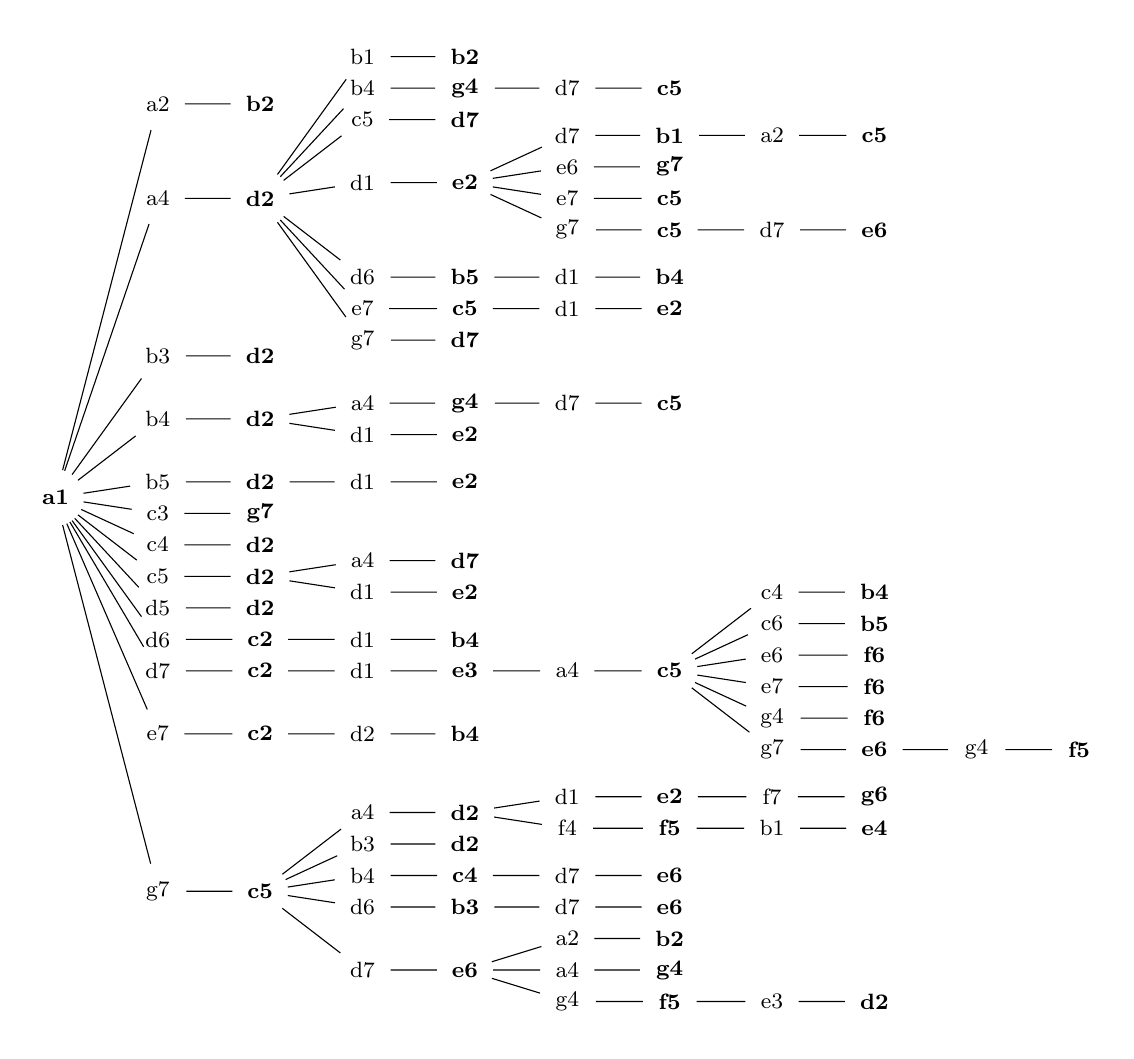
\begin{tikzpicture}[
	font=\footnotesize,
	grow'=right,
	level distance=13mm,
	level 1/.style={sibling distance=4mm},
	level 2/.style={sibling distance=4mm},
	level 3/.style={sibling distance=4mm},
	ww/.style={circle,font=\footnotesize\bfseries},
	wb/.style={circle},
	bw/.style={circle},
	bb/.style={circle,font=\footnotesize\bfseries},
	]
\node [ww] {a1}
	child { node [bw] {a2}
		child { node [ww] {b2} }
	}
	child [missing] foreach \a in {1,...,2} { }
	child { node [bw] {a4}
		child { node [ww] {d2}
			child { node [bw] {b1}
				child { node [ww] {b2} }
			}
			child { node [bw] {b4}
				child { node [ww] {g4}
					child { node [bw] {d7}
						child { node [ww] {c5} }
					}
				}
			}
			child { node [bw] {c5}
				child { node [ww] {d7} }
			}
			child [missing] foreach \a in {1,...,1} { }
			child { node [bw] {d1}
				child { node [ww] {e2}
					child { node [bw] {d7}
						child { node [ww] {b1}
							child { node [bw] {a2}
								child { node [ww] {c5} }
							}
						}
					}
					child { node [bw] {e6}
						child { node [ww] {g7} }
					}
					child { node [bw] {e7}
						child { node [ww] {c5} }
					}
					child { node [bw] {g7}
						child { node [ww] {c5}
							child { node [bw] {d7}
								child { node [ww] {e6} }
							}
						}
					}
				}
			}
			child [missing] foreach \a in {1,...,2} { }
			child { node [bw] {d6}
				child { node [ww] {b5}
					child { node [bw] {d1}
						child { node [ww] {b4} }
					}
				}
			}
			child { node [bw] {e7}
				child { node [ww] {c5}
					child { node [bw] {d1}
						child { node [ww] {e2} }
					}
				}
			}
			child { node [bw] {g7}
				child { node [ww] {d7} }
			}
		}
	}
	child [missing] foreach \a in {1,...,4} { }
	child { node [bw] {b3}
		child { node [ww] {d2} }
	}
	child [missing] foreach \a in {1,...,1} { }
	child { node [bw] {b4}
		child { node [ww] {d2}
			child { node [bw] {a4}
				child { node [ww] {g4}
					child { node [bw] {d7}
						child { node [ww] {c5} }
					}
				}
			}
			child { node [bw] {d1}
				child { node [ww] {e2} }
			}
		}
	}
	child [missing] foreach \a in {1,...,1} { }
	child { node [bw] {b5}
		child { node [ww] {d2}
			child { node [bw] {d1}
				child { node [ww] {e2} }
			}
		}
	}
	child { node [bw] {c3}
		child { node [ww] {g7} }
	}
	child { node [bw] {c4}
		child { node [ww] {d2} }
	}
	child { node [bw] {c5}
		child { node [ww] {d2}
			child { node [bw] {a4}
				child { node [ww] {d7} }
			}
			child { node [bw] {d1}
				child { node [ww] {e2} }
			}
		}
	}
	child { node [bw] {d5}
		child { node [ww] {d2} }
	}
	child { node [bw] {d6}
		child { node [ww] {c2}
			child { node [bw] {d1}
				child { node [ww] {b4} }
			}
		}
	}
	child { node [bw] {d7}
		child { node [ww] {c2}
			child { node [bw] {d1}
				child { node [ww] {e3}
					child { node [bw] {a4}
						child { node [ww] {c5}
							child { node [bw] {c4}
								child { node [ww] {b4} }
							}
							child { node [bw] {c6}
								child { node [ww] {b5} }
							}
							child { node [bw] {e6}
								child { node [ww] {f6} }
							}
							child { node [bw] {e7}
								child { node [ww] {f6} }
							}
							child { node [bw] {g4}
								child { node [ww] {f6} }
							}
							child { node [bw] {g7}
								child { node [ww] {e6}
									child { node [bw] {g4}
										child { node [ww] {f5} }
									}
								}
							}
						}
					}
				}
			}
		}
	}
	child [missing] foreach \a in {1,...,1} { }
	child { node [bw] {e7}
		child { node [ww] {c2}
			child { node [bw] {d2}
				child { node [ww] {b4} }
			}
		}
	}
	child [missing] foreach \a in {1,...,4} { }
	child { node [bw] {g7}
		child { node [ww] {c5}
			child { node [bw] {a4}
				child { node [ww] {d2}
					child { node [bw] {d1}
						child { node [ww] {e2}
							child { node [bw] {f7}
								child { node [ww] {g6} }
							}
						}
					}
					child { node [bw] {f4}
						child { node [ww] {f5}
							child { node [bw] {b1}
								child { node [ww] {e4} }
							}
						}
					}
				}
			}
			child { node [bw] {b3}
				child { node [ww] {d2} }
			}
			child { node [bw] {b4}
				child { node [ww] {c4}
					child { node [bw] {d7}
						child { node [ww] {e6} }
					}
				}
			}
			child { node [bw] {d6}
				child { node [ww] {b3}
					child { node [bw] {d7}
						child { node [ww] {e6} }
					}
				}
			}
			child [missing] foreach \a in {1,...,1} { }
			child { node [bw] {d7}
				child { node [ww] {e6}
					child { node [bw] {a2}
						child { node [ww] {b2} }
					}
					child { node [bw] {a4}
						child { node [ww] {g4} }
					}
					child { node [bw] {g4}
						child { node [ww] {f5}
							child { node [bw] {e3}
								child { node [ww] {d2} }
							}
						}
					}
				}
			}
		}
	}
;
\end{tikzpicture}


\caption{Proof Tree for the a1 opening on size 4 showing nodes that took more than 100 million simulations to solve}
\label{fig:proof-a1}
\end{figure}

\begin{figure}
\centering
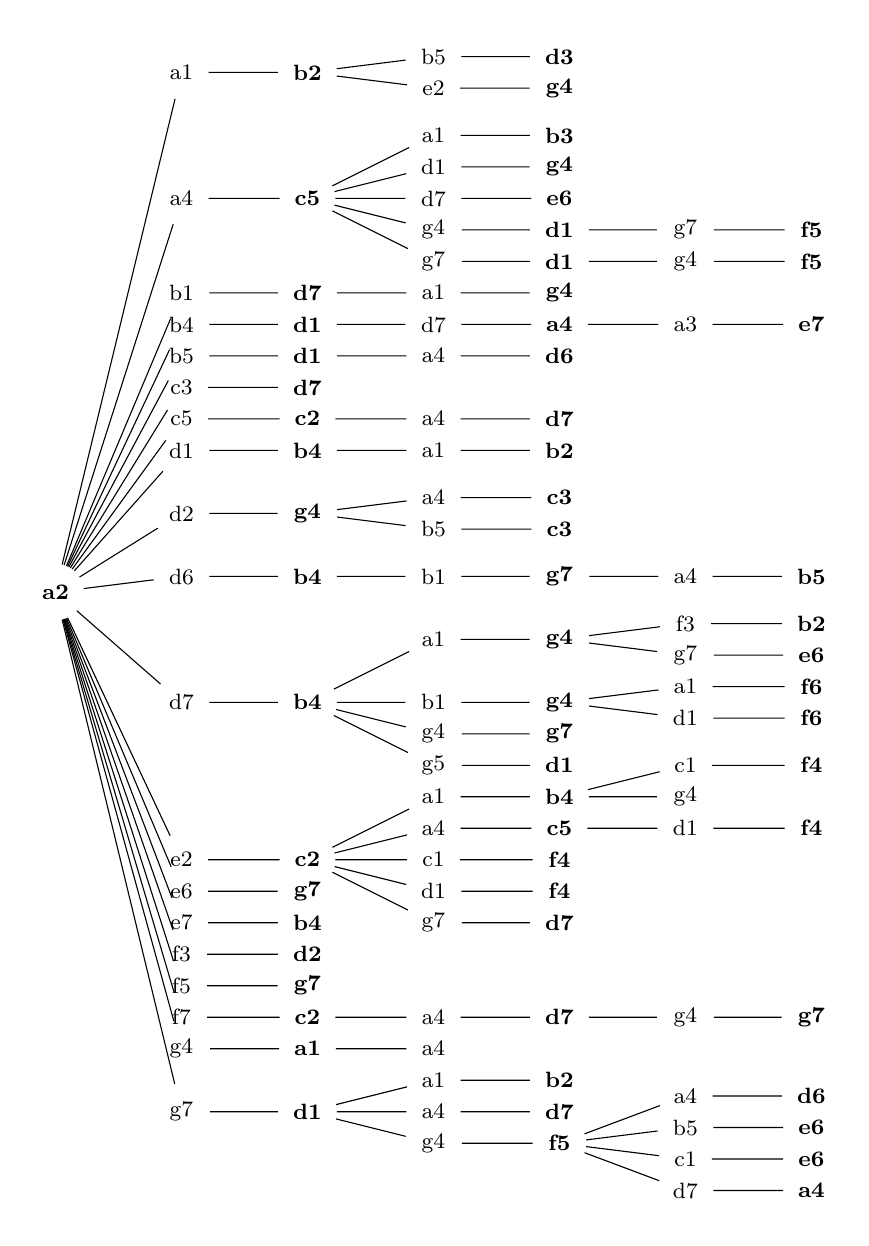
\begin{tikzpicture}[
	font=\footnotesize,
	grow'=right,
	level distance=16mm,
	level 1/.style={sibling distance=4mm},
	level 2/.style={sibling distance=4mm},
	level 3/.style={sibling distance=4mm},
	ww/.style={circle,font=\footnotesize\bfseries},
	wb/.style={circle},
	bw/.style={circle},
	bb/.style={circle,font=\footnotesize\bfseries},
	]
\node [ww] {a2}
	child { node [bw] {a1}
		child { node [ww] {b2}
			child { node [bw] {b5}
				child { node [ww] {d3}
				}
			}
			child { node [bw] {e2}
				child { node [ww] {g4}
				}
			}
		}
	}
	child [missing] foreach \a in {1,...,3} { }
	child { node [bw] {a4}
		child { node [ww] {c5}
			child { node [bw] {a1}
				child { node [ww] {b3}
				}
			}
			child { node [bw] {d1}
				child { node [ww] {g4}
				}
			}
			child { node [bw] {d7}
				child { node [ww] {e6}
				}
			}
			child { node [bw] {g4}
				child { node [ww] {d1}
					child { node [bw] {g7}
						child { node [ww] {f5}
						}
					}
				}
			}
			child { node [bw] {g7}
				child { node [ww] {d1}
					child { node [bw] {g4}
						child { node [ww] {f5}
						}
					}
				}
			}
		}
	}
	child [missing] foreach \a in {1,...,2} { }
	child { node [bw] {b1}
		child { node [ww] {d7}
			child { node [bw] {a1}
				child { node [ww] {g4}
				}
			}
		}
	}
	child { node [bw] {b4}
		child { node [ww] {d1}
			child { node [bw] {d7}
				child { node [ww] {a4}
					child { node [bw] {a3}
						child { node [ww] {e7}
						}
					}
				}
			}
		}
	}
	child { node [bw] {b5}
		child { node [ww] {d1}
			child { node [bw] {a4}
				child { node [ww] {d6}
				}
			}
		}
	}
	child { node [bw] {c3}
		child { node [ww] {d7}
		}
	}
	child { node [bw] {c5}
		child { node [ww] {c2}
			child { node [bw] {a4}
				child { node [ww] {d7}
				}
			}
		}
	}
	child { node [bw] {d1}
		child { node [ww] {b4}
			child { node [bw] {a1}
				child { node [ww] {b2}
				}
			}
		}
	}
	child [missing] foreach \a in {1,...,1} { }
	child { node [bw] {d2}
		child { node [ww] {g4}
			child { node [bw] {a4}
				child { node [ww] {c3}
				}
			}
			child { node [bw] {b5}
				child { node [ww] {c3}
				}
			}
		}
	}
	child [missing] foreach \a in {1,...,1} { }
	child { node [bw] {d6}
		child { node [ww] {b4}
			child { node [bw] {b1}
				child { node [ww] {g7}
					child { node [bw] {a4}
						child { node [ww] {b5}
						}
					}
				}
			}
		}
	}
	child [missing] foreach \a in {1,...,3} { }
	child { node [bw] {d7}
		child { node [ww] {b4}
			child { node [bw] {a1}
				child { node [ww] {g4}
					child { node [bw] {f3}
						child { node [ww] {b2}
						}
					}
					child { node [bw] {g7}
						child { node [ww] {e6}
						}
					}
				}
			}
			child [missing] foreach \a in {1,...,1} { }
			child { node [bw] {b1}
				child { node [ww] {g4}
					child { node [bw] {a1}
						child { node [ww] {f6}
						}
					}
					child { node [bw] {d1}
						child { node [ww] {f6}
						}
					}
				}
			}
			child { node [bw] {g4}
				child { node [ww] {g7}
				}
			}
			child { node [bw] {g5}
				child { node [ww] {d1}
				}
			}
		}
	}
	child [missing] foreach \a in {1,...,4} { }
	child { node [bw] {e2}
		child { node [ww] {c2}
			child { node [bw] {a1}
				child { node [ww] {b4}
					child { node [bw] {c1}
						child { node [ww] {f4}
						}
					}
					child { node [bw] {g4}
					}
					child [missing] foreach \a in {1,...,1} { }
				}
			}
			child { node [bw] {a4}
				child { node [ww] {c5}
					child { node [bw] {d1}
						child { node [ww] {f4}
						}
					}
				}
			}
			child { node [bw] {c1}
				child { node [ww] {f4}
				}
			}
			child { node [bw] {d1}
				child { node [ww] {f4}
				}
			}
			child { node [bw] {g7}
				child { node [ww] {d7}
				}
			}
		}
	}
	child { node [bw] {e6}
		child { node [ww] {g7}
		}
	}
	child { node [bw] {e7}
		child { node [ww] {b4}
		}
	}
	child { node [bw] {f3}
		child { node [ww] {d2}
		}
	}
	child { node [bw] {f5}
		child { node [ww] {g7}
		}
	}
	child { node [bw] {f7}
		child { node [ww] {c2}
			child { node [bw] {a4}
				child { node [ww] {d7}
					child { node [bw] {g4}
						child { node [ww] {g7}
						}
					}
				}
			}
		}
	}
	child { node [bw] {g4}
		child { node [ww] {a1}
			child { node [bw] {a4}
			}
		}
	}
	child [missing] foreach \a in {1,...,1} { }
	child { node [bw] {g7}
		child { node [ww] {d1}
			child { node [bw] {a1}
				child { node [ww] {b2}
				}
			}
			child { node [bw] {a4}
				child { node [ww] {d7}
				}
			}
			child { node [bw] {g4}
				child { node [ww] {f5}
					child { node [bw] {a4}
						child { node [ww] {d6}
						}
					}
					child { node [bw] {b5}
						child { node [ww] {e6}
						}
					}
					child { node [bw] {c1}
						child { node [ww] {e6}
						}
					}
					child { node [bw] {d7}
						child { node [ww] {a4}
						}
					}
				}
			}
		}
	}
;
\end{tikzpicture}


\caption{Proof Tree for the a2 opening on size 4 showing nodes that took more than 1 billion simulations to solve}
\label{fig:proof-a2}
\end{figure}

\begin{figure}
\centering
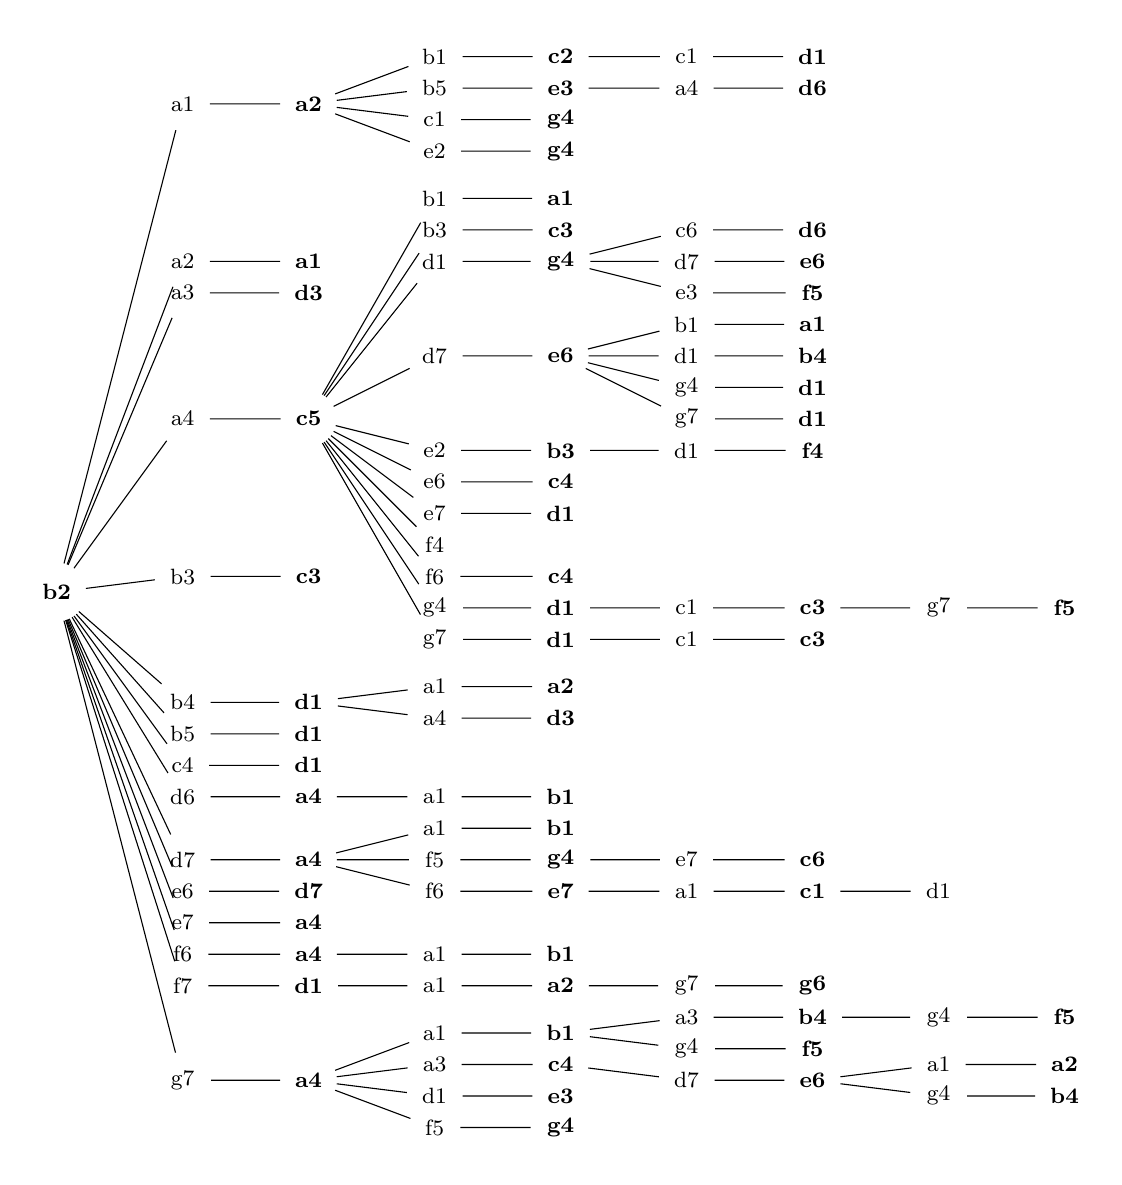
\begin{tikzpicture}[
	font=\footnotesize,
	grow'=right,
	level distance=16mm,
	level 1/.style={sibling distance=4mm},
	level 2/.style={sibling distance=4mm},
	level 3/.style={sibling distance=4mm},
	ww/.style={circle,font=\footnotesize\bfseries},
	wb/.style={circle},
	bw/.style={circle},
	bb/.style={circle,font=\footnotesize\bfseries},
	]
\node [ww] {b2}
	child { node [bw] {a1}
		child { node [ww] {a2}
			child { node [bw] {b1}
				child { node [ww] {c2}
					child { node [bw] {c1}
						child { node [ww] {d1}
						}
					}
				}
			}
			child { node [bw] {b5}
				child { node [ww] {e3}
					child { node [bw] {a4}
						child { node [ww] {d6}
						}
					}
				}
			}
			child { node [bw] {c1}
				child { node [ww] {g4}
				}
			}
			child { node [bw] {e2}
				child { node [ww] {g4}
				}
			}
		}
	}
	child [missing] foreach \a in {1,...,4} { }
	child { node [bw] {a2}
		child { node [ww] {a1}
		}
	}
	child { node [bw] {a3}
		child { node [ww] {d3}
		}
	}
	child [missing] foreach \a in {1,...,3} { }
	child { node [bw] {a4}
		child { node [ww] {c5}
			child { node [bw] {b1}
				child { node [ww] {a1}
				}
			}
			child { node [bw] {b3}
				child { node [ww] {c3}
				}
			}
			child { node [bw] {d1}
				child { node [ww] {g4}
					child { node [bw] {c6}
						child { node [ww] {d6}
						}
					}
					child { node [bw] {d7}
						child { node [ww] {e6}
						}
					}
					child { node [bw] {e3}
						child { node [ww] {f5}
						}
					}
				}
			}
			child [missing] foreach \a in {1,...,2} { }
			child { node [bw] {d7}
				child { node [ww] {e6}
					child [missing] foreach \a in {1,...,1} { }
					child { node [bw] {b1}
						child { node [ww] {a1}
						}
					}
					child { node [bw] {d1}
						child { node [ww] {b4}
						}
					}
					child { node [bw] {g4}
						child { node [ww] {d1}
						}
					}
					child { node [bw] {g7}
						child { node [ww] {d1}
						}
					}
				}
			}
			child [missing] foreach \a in {1,...,2} { }
			child { node [bw] {e2}
				child { node [ww] {b3}
					child { node [bw] {d1}
						child { node [ww] {f4}
						}
					}
				}
			}
			child { node [bw] {e6}
				child { node [ww] {c4}
				}
			}
			child { node [bw] {e7}
				child { node [ww] {d1}
				}
			}
			child { node [bw] {f4}
			}
			child { node [bw] {f6}
				child { node [ww] {c4}
				}
			}
			child { node [bw] {g4}
				child { node [ww] {d1}
					child { node [bw] {c1}
						child { node [ww] {c3}
							child { node [bw] {g7}
								child { node [ww] {f5}
								}
							}
						}
					}
				}
			}
			child { node [bw] {g7}
				child { node [ww] {d1}
					child { node [bw] {c1}
						child { node [ww] {c3}
						}
					}
				}
			}
		}
	}
	child [missing] foreach \a in {1,...,4} { }
	child { node [bw] {b3}
		child { node [ww] {c3}
		}
	}
	child [missing] foreach \a in {1,...,3} { }
	child { node [bw] {b4}
		child { node [ww] {d1}
			child { node [bw] {a1}
				child { node [ww] {a2}
				}
			}
			child { node [bw] {a4}
				child { node [ww] {d3}
				}
			}
		}
	}
	child { node [bw] {b5}
		child { node [ww] {d1}
		}
	}
	child { node [bw] {c4}
		child { node [ww] {d1}
		}
	}
	child { node [bw] {d6}
		child { node [ww] {a4}
			child { node [bw] {a1}
				child { node [ww] {b1}
				}
			}
		}
	}
	child [missing] foreach \a in {1,...,1} { }
	child { node [bw] {d7}
		child { node [ww] {a4}
			child { node [bw] {a1}
				child { node [ww] {b1}
				}
			}
			child { node [bw] {f5}
				child { node [ww] {g4}
					child { node [bw] {e7}
						child { node [ww] {c6}
						}
					}
				}
			}
			child { node [bw] {f6}
				child { node [ww] {e7}
					child { node [bw] {a1}
						child { node [ww] {c1}
							child { node [bw] {d1}
							}
						}
					}
				}
			}
		}
	}
	child { node [bw] {e6}
		child { node [ww] {d7}
		}
	}
	child { node [bw] {e7}
		child { node [ww] {a4}
		}
	}
	child { node [bw] {f6}
		child { node [ww] {a4}
			child { node [bw] {a1}
				child { node [ww] {b1}
				}
			}
		}
	}
	child { node [bw] {f7}
		child { node [ww] {d1}
			child { node [bw] {a1}
				child { node [ww] {a2}
					child { node [bw] {g7}
						child { node [ww] {g6}
						}
					}
				}
			}
		}
	}
	child [missing] foreach \a in {1,...,2} { }
	child { node [bw] {g7}
		child { node [ww] {a4}
			child { node [bw] {a1}
				child { node [ww] {b1}
					child { node [bw] {a3}
						child { node [ww] {b4}
							child { node [bw] {g4}
								child { node [ww] {f5}
								}
							}
						}
					}
					child { node [bw] {g4}
						child { node [ww] {f5}
						}
					}
				}
			}
			child { node [bw] {a3}
				child { node [ww] {c4}
					child [missing] foreach \a in {1,...,1} { }
					child { node [bw] {d7}
						child { node [ww] {e6}
							child { node [bw] {a1}
								child { node [ww] {a2}
								}
							}
							child { node [bw] {g4}
								child { node [ww] {b4}
								}
							}
						}
					}
				}
			}
			child { node [bw] {d1}
				child { node [ww] {e3}
				}
			}
			child { node [bw] {f5}
				child { node [ww] {g4}
				}
			}
		}
	}
;
\end{tikzpicture}


\caption{Proof Tree for the b2 opening on size 4 showing nodes that took more than 250 million simulations to solve}
\label{fig:proof-b2}
\end{figure}

\begin{figure}
\centering
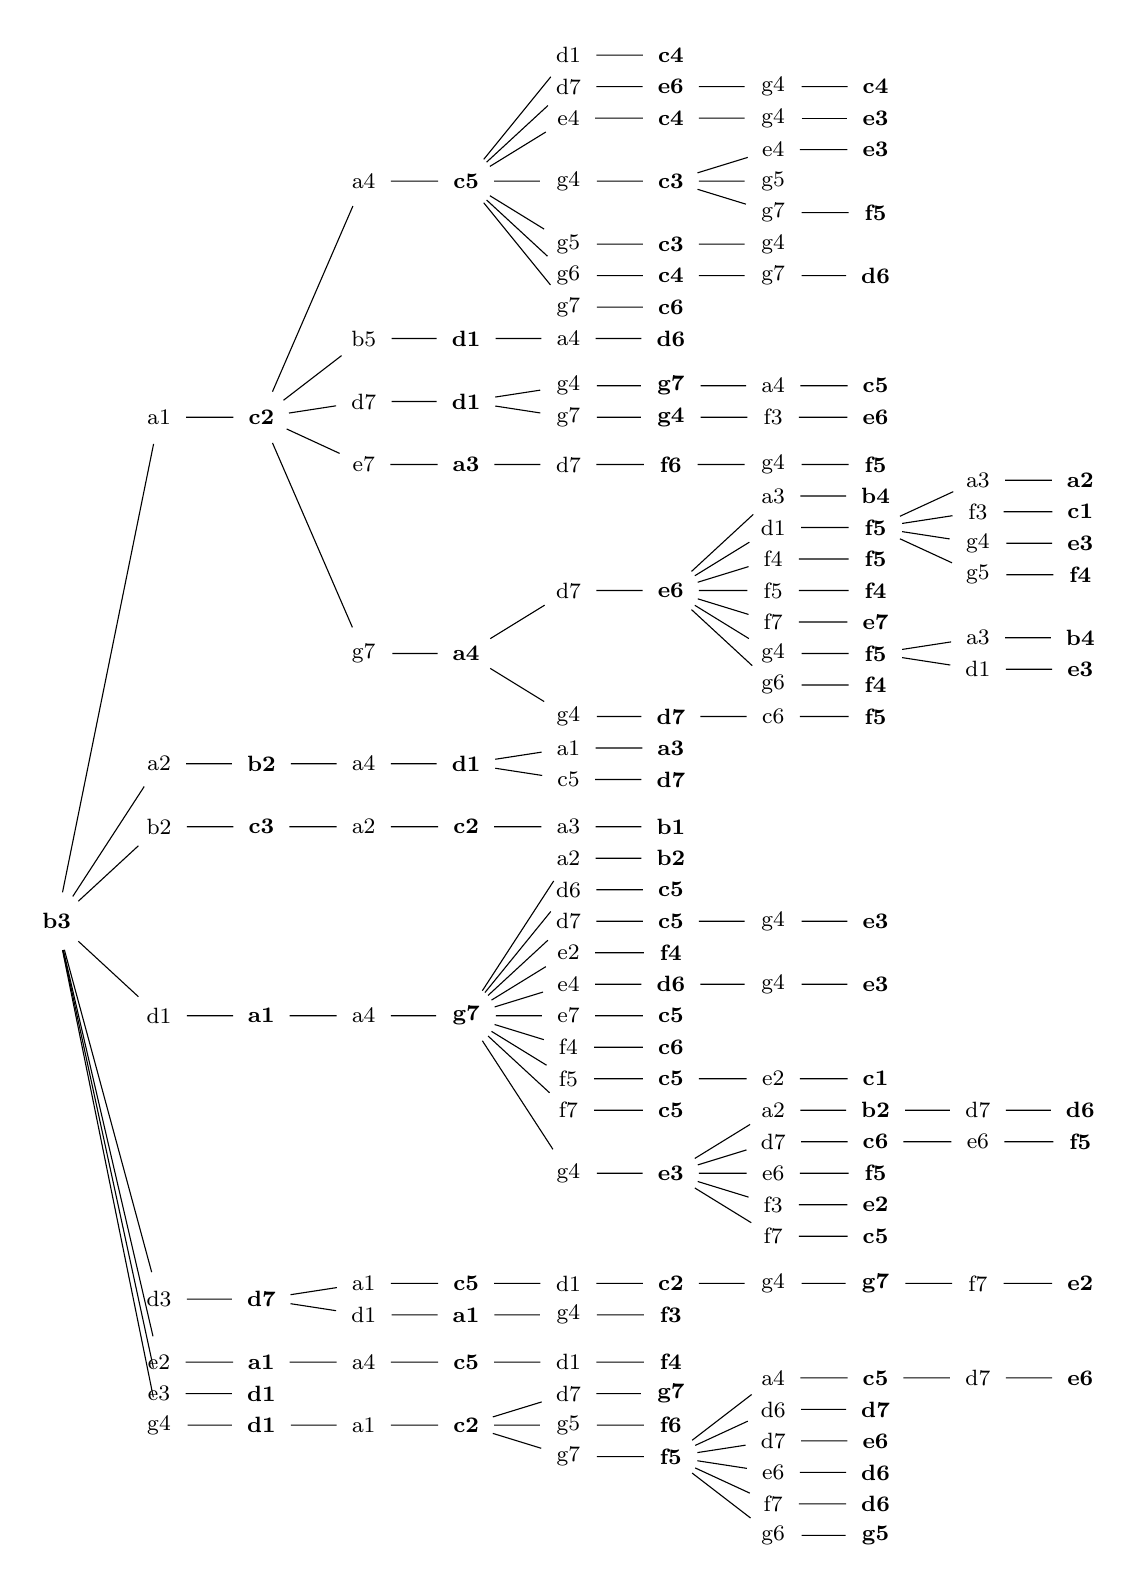
\begin{tikzpicture}[
	font=\footnotesize,
	grow'=right,
	level distance=13mm,
	level 1/.style={sibling distance=4mm},
	level 2/.style={sibling distance=4mm},
	level 3/.style={sibling distance=4mm},
	ww/.style={circle,font=\footnotesize\bfseries},
	wb/.style={circle},
	bw/.style={circle},
	bb/.style={circle,font=\footnotesize\bfseries},
	]
\node [ww] {b3}
	child { node [bw] {a1}
		child { node [ww] {c2}
			child { node [bw] {a4}
				child { node [ww] {c5}
					child { node [bw] {d1}
						child { node [ww] {c4}
						}
					}
					child { node [bw] {d7}
						child { node [ww] {e6}
							child { node [bw] {g4}
								child { node [ww] {c4}
								}
							}
						}
					}
					child { node [bw] {e4}
						child { node [ww] {c4}
							child { node [bw] {g4}
								child { node [ww] {e3}
								}
							}
						}
					}
					child [missing] foreach \a in {1,...,1} { }
					child { node [bw] {g4}
						child { node [ww] {c3}
							child { node [bw] {e4}
								child { node [ww] {e3}
								}
							}
							child { node [bw] {g5}
							}
							child { node [bw] {g7}
								child { node [ww] {f5}
								}
							}
						}
					}
					child [missing] foreach \a in {1,...,1} { }
					child { node [bw] {g5}
						child { node [ww] {c3}
							child { node [bw] {g4}
							}
						}
					}
					child { node [bw] {g6}
						child { node [ww] {c4}
							child { node [bw] {g7}
								child { node [ww] {d6}
								}
							}
						}
					}
					child { node [bw] {g7}
						child { node [ww] {c6}
						}
					}
				}
			}
			child [missing] foreach \a in {1,...,4} { }
			child { node [bw] {b5}
				child { node [ww] {d1}
					child { node [bw] {a4}
						child { node [ww] {d6}
						}
					}
				}
			}
			child [missing] foreach \a in {1,...,1} { }
			child { node [bw] {d7}
				child { node [ww] {d1}
					child { node [bw] {g4}
						child { node [ww] {g7}
							child { node [bw] {a4}
								child { node [ww] {c5}
								}
							}
						}
					}
					child { node [bw] {g7}
						child { node [ww] {g4}
							child { node [bw] {f3}
								child { node [ww] {e6}
								}
							}
						}
					}
				}
			}
			child [missing] foreach \a in {1,...,1} { }
			child { node [bw] {e7}
				child { node [ww] {a3}
					child { node [bw] {d7}
						child { node [ww] {f6}
							child { node [bw] {g4}
								child { node [ww] {f5}
								}
							}
						}
					}
				}
			}
			child [missing] foreach \a in {1,...,5} { }
			child { node [bw] {g7}
				child { node [ww] {a4}
					child { node [bw] {d7}
						child { node [ww] {e6}
							child { node [bw] {a3}
								child { node [ww] {b4}
								}
							}
							child { node [bw] {d1}
								child { node [ww] {f5}
									child { node [bw] {a3}
										child { node [ww] {a2}
										}
									}
									child { node [bw] {f3}
										child { node [ww] {c1}
										}
									}
									child { node [bw] {g4}
										child { node [ww] {e3}
										}
									}
									child { node [bw] {g5}
										child { node [ww] {f4}
										}
									}
								}
							}
							child { node [bw] {f4}
								child { node [ww] {f5}
								}
							}
							child { node [bw] {f5}
								child { node [ww] {f4}
								}
							}
							child { node [bw] {f7}
								child { node [ww] {e7}
								}
							}
							child { node [bw] {g4}
								child { node [ww] {f5}
									child { node [bw] {a3}
										child { node [ww] {b4}
										}
									}
									child { node [bw] {d1}
										child { node [ww] {e3}
										}
									}
								}
							}
							child { node [bw] {g6}
								child { node [ww] {f4}
								}
							}
						}
					}
					child [missing] foreach \a in {1,...,3} { }
					child { node [bw] {g4}
						child { node [ww] {d7}
							child { node [bw] {c6}
								child { node [ww] {f5}
								}
							}
						}
					}
				}
			}
		}
	}
	child [missing] foreach \a in {1,...,10} { }
	child { node [bw] {a2}
		child { node [ww] {b2}
			child { node [bw] {a4}
				child { node [ww] {d1}
					child { node [bw] {a1}
						child { node [ww] {a3}
						}
					}
					child { node [bw] {c5}
						child { node [ww] {d7}
						}
					}
%					child [missing] foreach \a in {1,...,1} { }
				}
			}
		}
	}
	child [missing] foreach \a in {1,...,1} { }
	child { node [bw] {b2}
		child { node [ww] {c3}
			child { node [bw] {a2}
				child { node [ww] {c2}
					child { node [bw] {a3}
						child { node [ww] {b1}
						}
					}
				}
			}
		}
	}
	child [missing] foreach \a in {1,...,5} { }
	child { node [bw] {d1}
		child { node [ww] {a1}
			child { node [bw] {a4}
				child { node [ww] {g7}
					child { node [bw] {a2}
						child { node [ww] {b2}
						}
					}
					child { node [bw] {d6}
						child { node [ww] {c5}
						}
					}
					child { node [bw] {d7}
						child { node [ww] {c5}
							child { node [bw] {g4}
								child { node [ww] {e3}
								}
							}
						}
					}
					child { node [bw] {e2}
						child { node [ww] {f4}
						}
					}
					child { node [bw] {e4}
						child { node [ww] {d6}
							child { node [bw] {g4}
								child { node [ww] {e3}
								}
							}
						}
					}
					child { node [bw] {e7}
						child { node [ww] {c5}
						}
					}
					child { node [bw] {f4}
						child { node [ww] {c6}
						}
					}
					child { node [bw] {f5}
						child { node [ww] {c5}
							child { node [bw] {e2}
								child { node [ww] {c1}
								}
							}
						}
					}
					child { node [bw] {f7}
						child { node [ww] {c5}
						}
					}
					child [missing] foreach \a in {1,...,1} { }
					child { node [bw] {g4}
						child { node [ww] {e3}
							child { node [bw] {a2}
								child { node [ww] {b2}
									child { node [bw] {d7}
										child { node [ww] {d6}
										}
									}
								}
							}
							child { node [bw] {d7}
								child { node [ww] {c6}
									child { node [bw] {e6}
										child { node [ww] {f5}
										}
									}
								}
							}
							child { node [bw] {e6}
								child { node [ww] {f5}
								}
							}
							child { node [bw] {f3}
								child { node [ww] {e2}
								}
							}
							child { node [bw] {f7}
								child { node [ww] {c5}
								}
							}
						}
					}
				}
			}
		}
	}
	child [missing] foreach \a in {1,...,8} { }
	child { node [bw] {d3}
		child { node [ww] {d7}
			child { node [bw] {a1}
				child { node [ww] {c5}
					child { node [bw] {d1}
						child { node [ww] {c2}
							child { node [bw] {g4}
								child { node [ww] {g7}
									child { node [bw] {f7}
										child { node [ww] {e2}
										}
									}
								}
							}
						}
					}
				}
			}
			child { node [bw] {d1}
				child { node [ww] {a1}
					child { node [bw] {g4}
						child { node [ww] {f3}
						}
					}
				}
			}
		}
	}
	child [missing] foreach \a in {1,...,1} { }
	child { node [bw] {e2}
		child { node [ww] {a1}
			child { node [bw] {a4}
				child { node [ww] {c5}
					child { node [bw] {d1}
						child { node [ww] {f4}
						}
					}
				}
			}
		}
	}
	child { node [bw] {e3}
		child { node [ww] {d1}
		}
	}
	child { node [bw] {g4}
		child { node [ww] {d1}
			child { node [bw] {a1}
				child { node [ww] {c2}
					child { node [bw] {d7}
						child { node [ww] {g7}
						}
					}
					child { node [bw] {g5}
						child { node [ww] {f6}
						}
					}
					child { node [bw] {g7}
						child { node [ww] {f5}
							child { node [bw] {a4}
								child { node [ww] {c5}
									child { node [bw] {d7}
										child { node [ww] {e6}
										}
									}
								}
							}
							child { node [bw] {d6}
								child { node [ww] {d7}
								}
							}
							child { node [bw] {d7}
								child { node [ww] {e6}
								}
							}
							child { node [bw] {e6}
								child { node [ww] {d6}
								}
							}
							child { node [bw] {f7}
								child { node [ww] {d6}
								}
							}
							child { node [bw] {g6}
								child { node [ww] {g5}
								}
							}
						}
					}
				}
			}
		}
	}
;
\end{tikzpicture}


\caption{Proof Tree for the b3 opening on size 4 showing nodes that took more than 100 million simulations to solve}
\label{fig:proof-b3}
\end{figure}

\begin{figure}
\centering
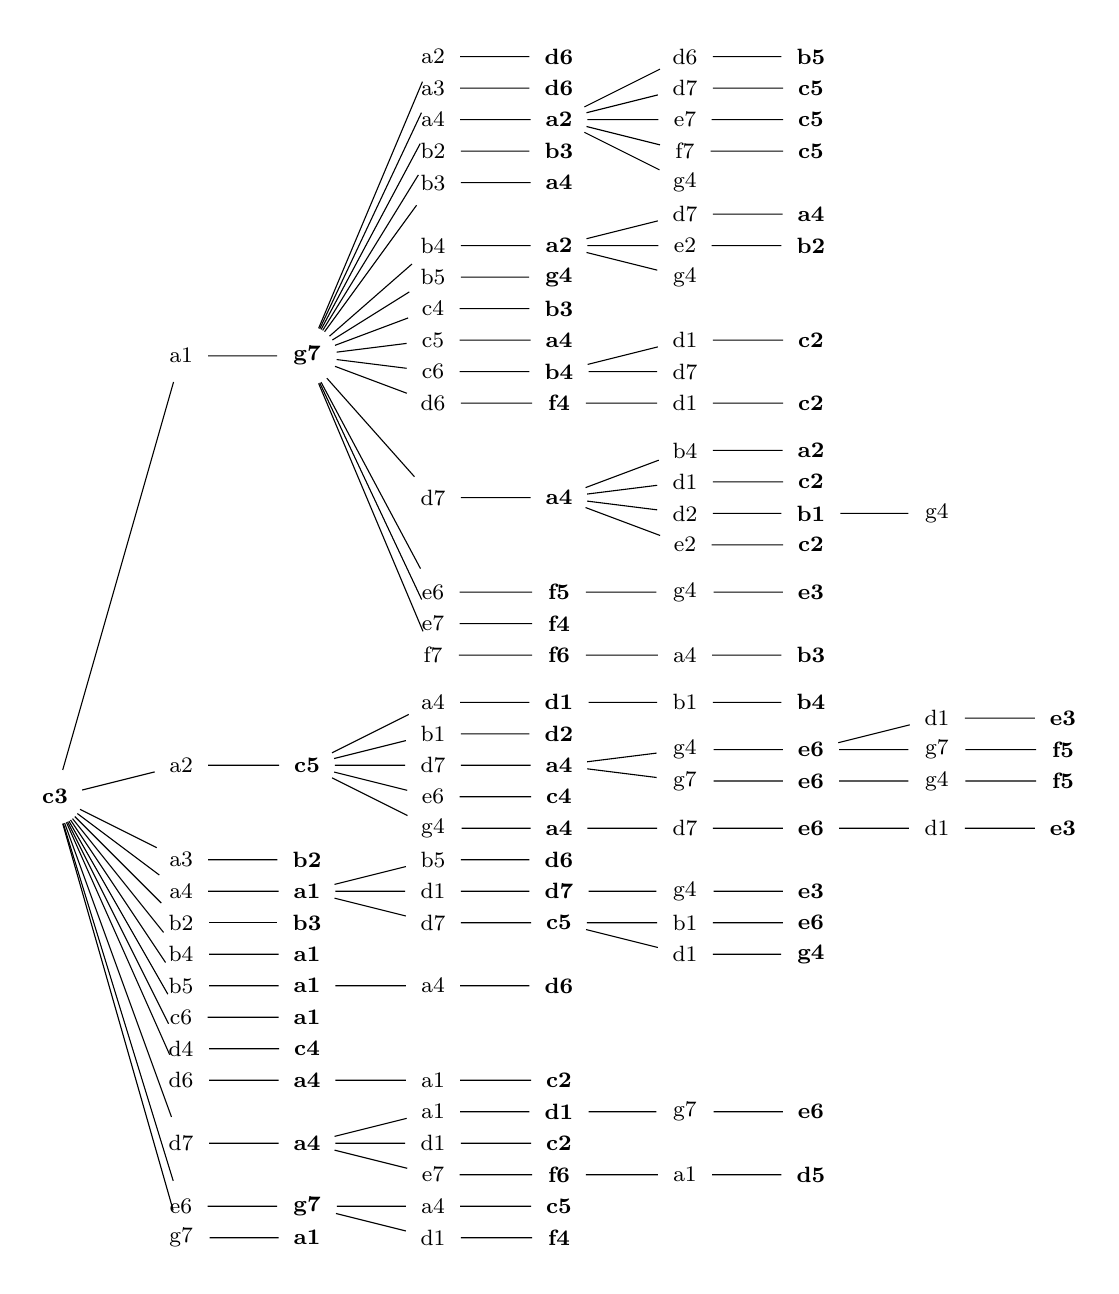
\begin{tikzpicture}[
	font=\footnotesize,
	grow'=right,
	level distance=16mm,
	level 1/.style={sibling distance=4mm},
	level 2/.style={sibling distance=4mm},
	level 3/.style={sibling distance=4mm},
	ww/.style={circle,font=\footnotesize\bfseries},
	wb/.style={circle},
	bw/.style={circle},
	bb/.style={circle,font=\footnotesize\bfseries},
	]
\node [ww] {c3}
	child { node [bw] {a1}
		child { node [ww] {g7}
			child { node [bw] {a2}
				child { node [ww] {d6}
				}
			}
			child { node [bw] {a3}
				child { node [ww] {d6}
				}
			}
			child { node [bw] {a4}
				child { node [ww] {a2}
					child { node [bw] {d6}
						child { node [ww] {b5}
						}
					}
					child { node [bw] {d7}
						child { node [ww] {c5}
						}
					}
					child { node [bw] {e7}
						child { node [ww] {c5}
						}
					}
					child { node [bw] {f7}
						child { node [ww] {c5}
						}
					}
					child { node [bw] {g4}
					}
				}
			}
			child { node [bw] {b2}
				child { node [ww] {b3}
				}
			}
			child { node [bw] {b3}
				child { node [ww] {a4}
				}
			}
			child [missing] foreach \a in {1,...,1} { }
			child { node [bw] {b4}
				child { node [ww] {a2}
					child { node [bw] {d7}
						child { node [ww] {a4}
						}
					}
					child { node [bw] {e2}
						child { node [ww] {b2}
						}
					}
					child { node [bw] {g4}
					}
				}
			}
			child { node [bw] {b5}
				child { node [ww] {g4}
				}
			}
			child { node [bw] {c4}
				child { node [ww] {b3}
				}
			}
			child { node [bw] {c5}
				child { node [ww] {a4}
				}
			}
			child { node [bw] {c6}
				child { node [ww] {b4}
					child { node [bw] {d1}
						child { node [ww] {c2}
						}
					}
					child { node [bw] {d7}
					}
					child [missing] foreach \a in {1,...,1} { }
				}
			}
			child { node [bw] {d6}
				child { node [ww] {f4}
					child { node [bw] {d1}
						child { node [ww] {c2}
						}
					}
				}
			}
			child [missing] foreach \a in {1,...,2} { }
			child { node [bw] {d7}
				child { node [ww] {a4}
					child { node [bw] {b4}
						child { node [ww] {a2}
						}
					}
					child { node [bw] {d1}
						child { node [ww] {c2}
						}
					}
					child { node [bw] {d2}
						child { node [ww] {b1}
							child { node [bw] {g4}
							}
						}
					}
					child { node [bw] {e2}
						child { node [ww] {c2}
						}
					}
				}
			}
			child [missing] foreach \a in {1,...,2} { }
			child { node [bw] {e6}
				child { node [ww] {f5}
					child { node [bw] {g4}
						child { node [ww] {e3}
						}
					}
				}
			}
			child { node [bw] {e7}
				child { node [ww] {f4}
				}
			}
			child { node [bw] {f7}
				child { node [ww] {f6}
					child { node [bw] {a4}
						child { node [ww] {b3}
						}
					}
				}
			}
		}
	}
	child [missing] foreach \a in {1,...,12} { }
	child { node [bw] {a2}
		child { node [ww] {c5}
			child { node [bw] {a4}
				child { node [ww] {d1}
					child { node [bw] {b1}
						child { node [ww] {b4}
						}
					}
				}
			}
			child { node [bw] {b1}
				child { node [ww] {d2}
				}
			}
			child { node [bw] {d7}
				child { node [ww] {a4}
					child { node [bw] {g4}
						child { node [ww] {e6}
							child { node [bw] {d1}
								child { node [ww] {e3}
								}
							}
							child { node [bw] {g7}
								child { node [ww] {f5}
								}
							}
							child [missing] foreach \a in {1,...,1} { }
						}
					}
					child { node [bw] {g7}
						child { node [ww] {e6}
							child { node [bw] {g4}
								child { node [ww] {f5}
								}
							}
						}
					}
				}
			}
			child { node [bw] {e6}
				child { node [ww] {c4}
				}
			}
			child { node [bw] {g4}
				child { node [ww] {a4}
					child { node [bw] {d7}
						child { node [ww] {e6}
							child { node [bw] {d1}
								child { node [ww] {e3}
								}
							}
						}
					}
				}
			}
		}
	}
	child [missing] foreach \a in {1,...,2} { }
	child { node [bw] {a3}
		child { node [ww] {b2}
		}
	}
	child { node [bw] {a4}
		child { node [ww] {a1}
			child { node [bw] {b5}
				child { node [ww] {d6}
				}
			}
			child { node [bw] {d1}
				child { node [ww] {d7}
					child { node [bw] {g4}
						child { node [ww] {e3}
						}
					}
				}
			}
			child { node [bw] {d7}
				child { node [ww] {c5}
					child [missing] foreach \a in {1,...,1} { }
					child { node [bw] {b1}
						child { node [ww] {e6}
						}
					}
					child { node [bw] {d1}
						child { node [ww] {g4}
						}
					}
				}
			}
		}
	}
	child { node [bw] {b2}
		child { node [ww] {b3}
		}
	}
	child { node [bw] {b4}
		child { node [ww] {a1}
		}
	}
	child { node [bw] {b5}
		child { node [ww] {a1}
			child { node [bw] {a4}
				child { node [ww] {d6}
				}
			}
		}
	}
	child { node [bw] {c6}
		child { node [ww] {a1}
		}
	}
	child { node [bw] {d4}
		child { node [ww] {c4}
		}
	}
	child { node [bw] {d6}
		child { node [ww] {a4}
			child { node [bw] {a1}
				child { node [ww] {c2}
				}
			}
		}
	}
	child [missing] foreach \a in {1,...,1} { }
	child { node [bw] {d7}
		child { node [ww] {a4}
			child { node [bw] {a1}
				child { node [ww] {d1}
					child { node [bw] {g7}
						child { node [ww] {e6}
						}
					}
				}
			}
			child { node [bw] {d1}
				child { node [ww] {c2}
				}
			}
			child { node [bw] {e7}
				child { node [ww] {f6}
					child { node [bw] {a1}
						child { node [ww] {d5}
						}
					}
				}
			}
		}
	}
	child [missing] foreach \a in {1,...,1} { }
	child { node [bw] {e6}
		child { node [ww] {g7}
			child [missing] foreach \a in {1,...,1} { }
			child { node [bw] {a4}
				child { node [ww] {c5}
				}
			}
			child { node [bw] {d1}
				child { node [ww] {f4}
				}
			}
		}
	}
	child { node [bw] {g7}
		child { node [ww] {a1}
		}
	}
;
\end{tikzpicture}


\caption{Proof Tree for the c3 opening on size 4 showing nodes that took more than 600 million simulations to solve}
\label{fig:proof-c3}
\end{figure}

\begin{figure}
\centering
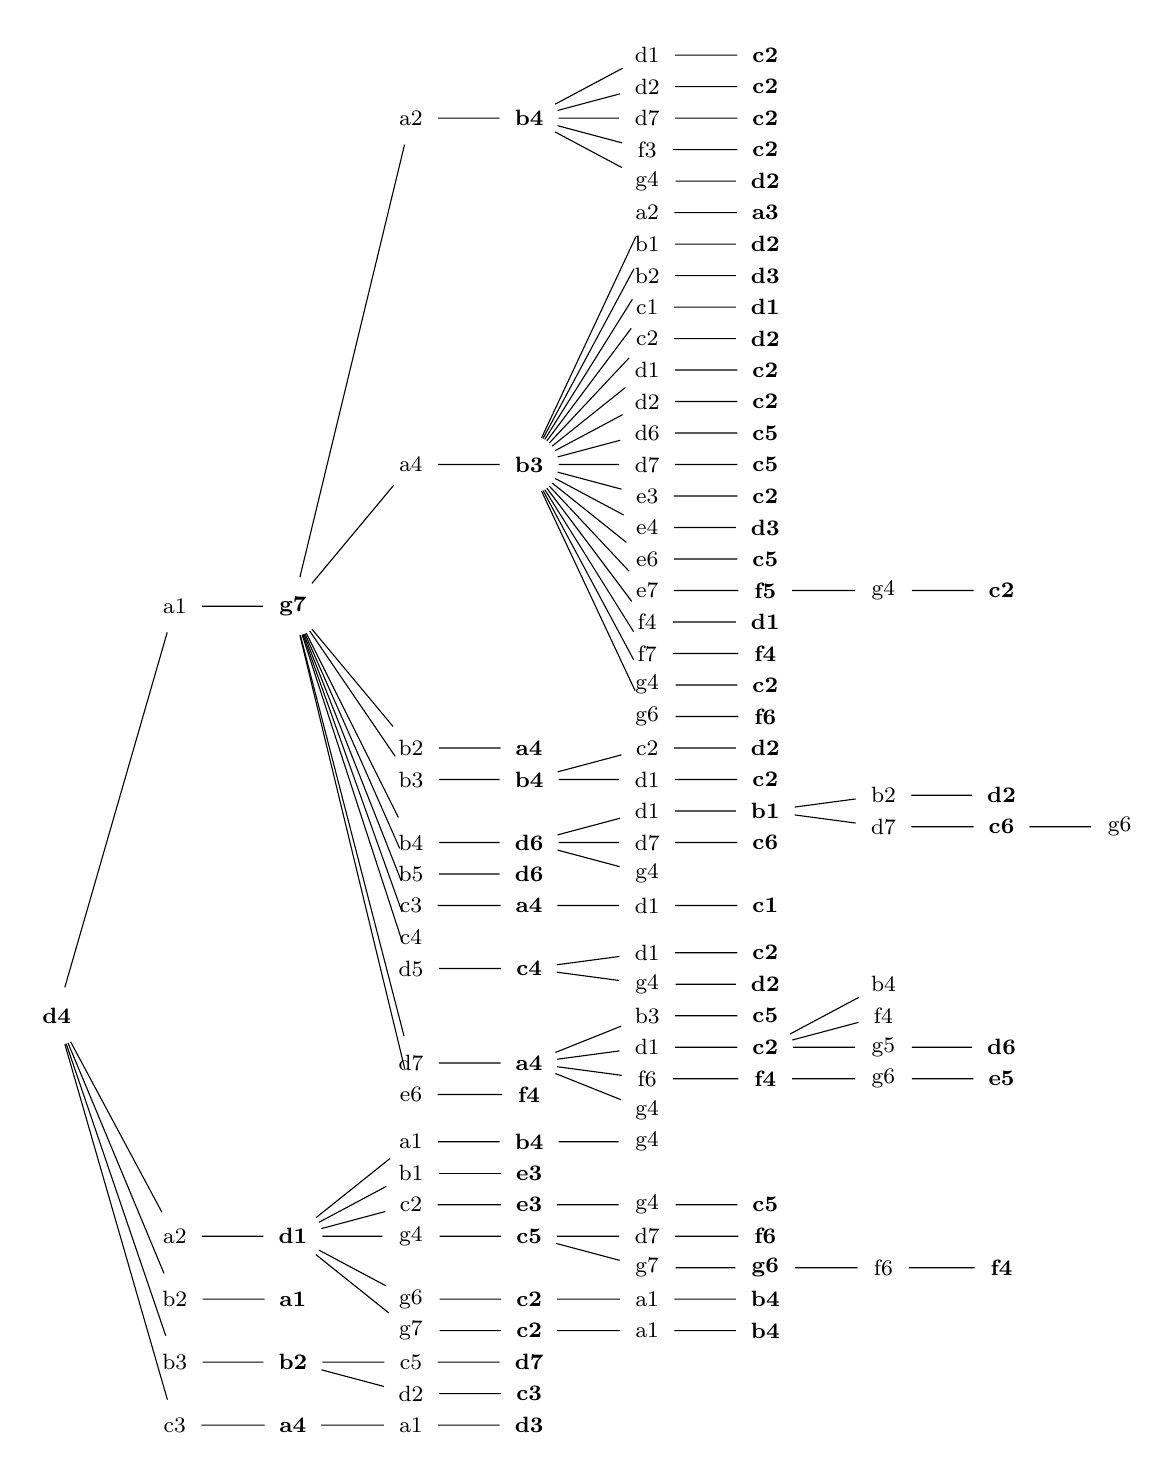
\begin{tikzpicture}[
	font=\footnotesize,
	grow'=right,
	level distance=15mm,
	level 1/.style={sibling distance=4mm},
	level 2/.style={sibling distance=4mm},
	level 3/.style={sibling distance=4mm},
	ww/.style={circle,font=\footnotesize\bfseries},
	wb/.style={circle},
	bw/.style={circle},
	bb/.style={circle,font=\footnotesize\bfseries},
	]
\node [ww] {d4}
	child { node [bw] {a1}
		child { node [ww] {g7}
			child { node [bw] {a2}
				child { node [ww] {b4}
					child { node [bw] {d1}
						child { node [ww] {c2}
						}
					}
					child { node [bw] {d2}
						child { node [ww] {c2}
						}
					}
					child { node [bw] {d7}
						child { node [ww] {c2}
						}
					}
					child { node [bw] {f3}
						child { node [ww] {c2}
						}
					}
					child { node [bw] {g4}
						child { node [ww] {d2}
						}
					}
				}
			}
			child [missing] foreach \a in {1,...,10} { }
			child { node [bw] {a4}
				child { node [ww] {b3}
					child { node [bw] {a2}
						child { node [ww] {a3}
						}
					}
					child { node [bw] {b1}
						child { node [ww] {d2}
						}
					}
					child { node [bw] {b2}
						child { node [ww] {d3}
						}
					}
					child { node [bw] {c1}
						child { node [ww] {d1}
						}
					}
					child { node [bw] {c2}
						child { node [ww] {d2}
						}
					}
					child { node [bw] {d1}
						child { node [ww] {c2}
						}
					}
					child { node [bw] {d2}
						child { node [ww] {c2}
						}
					}
					child { node [bw] {d6}
						child { node [ww] {c5}
						}
					}
					child { node [bw] {d7}
						child { node [ww] {c5}
						}
					}
					child { node [bw] {e3}
						child { node [ww] {c2}
						}
					}
					child { node [bw] {e4}
						child { node [ww] {d3}
						}
					}
					child { node [bw] {e6}
						child { node [ww] {c5}
						}
					}
					child { node [bw] {e7}
						child { node [ww] {f5}
							child { node [bw] {g4}
								child { node [ww] {c2}
								}
							}
						}
					}
					child { node [bw] {f4}
						child { node [ww] {d1}
						}
					}
					child { node [bw] {f7}
						child { node [ww] {f4}
						}
					}
					child { node [bw] {g4}
						child { node [ww] {c2}
						}
					}
					child { node [bw] {g6}
						child { node [ww] {f6}
						}
					}
				}
			}
			child [missing] foreach \a in {1,...,8} { }
			child { node [bw] {b2}
				child { node [ww] {a4}
				}
			}
			child { node [bw] {b3}
				child { node [ww] {b4}
					child { node [bw] {c2}
						child { node [ww] {d2}
						}
					}
					child { node [bw] {d1}
						child { node [ww] {c2}
						}
					}
					child [missing] foreach \a in {1,...,1} { }
				}
			}
			child [missing] foreach \a in {1,...,1} { }
			child { node [bw] {b4}
				child { node [ww] {d6}
					child { node [bw] {d1}
						child { node [ww] {b1}
							child { node [bw] {b2}
								child { node [ww] {d2}
								}
							}
							child { node [bw] {d7}
								child { node [ww] {c6}
									child { node [bw] {g6}
									}
								}
							}
						}
					}
					child { node [bw] {d7}
						child { node [ww] {c6}
						}
					}
					child { node [bw] {g4}
					}
				}
			}
			child { node [bw] {b5}
				child { node [ww] {d6}
				}
			}
			child { node [bw] {c3}
				child { node [ww] {a4}
					child { node [bw] {d1}
						child { node [ww] {c1}
						}
					}
				}
			}
			child { node [bw] {c4}
			}
			child { node [bw] {d5}
				child { node [ww] {c4}
					child { node [bw] {d1}
						child { node [ww] {c2}
						}
					}
					child { node [bw] {g4}
						child { node [ww] {d2}
						}
					}
				}
			}
			child [missing] foreach \a in {1,...,2} { }
			child { node [bw] {d7}
				child { node [ww] {a4}
					child { node [bw] {b3}
						child { node [ww] {c5}
						}
					}
					child { node [bw] {d1}
						child { node [ww] {c2}
							child { node [bw] {b4}
							}
							child { node [bw] {f4}
							}
							child { node [bw] {g5}
								child { node [ww] {d6}
								}
							}
							child [missing] foreach \a in {1,...,2} { }
						}
					}
					child { node [bw] {f6}
						child { node [ww] {f4}
							child { node [bw] {g6}
								child { node [ww] {e5}
								}
							}
						}
					}
					child { node [bw] {g4}
					}
				}
			}
			child { node [bw] {e6}
				child { node [ww] {f4}
				}
			}
		}
	}
	child [missing] foreach \a in {1,...,19} { }
	child { node [bw] {a2}
		child { node [ww] {d1}
			child { node [bw] {a1}
				child { node [ww] {b4}
					child { node [bw] {g4}
					}
				}
			}
			child { node [bw] {b1}
				child { node [ww] {e3}
				}
			}
			child { node [bw] {c2}
				child { node [ww] {e3}
					child { node [bw] {g4}
						child { node [ww] {c5}
						}
					}
				}
			}
			child { node [bw] {g4}
				child { node [ww] {c5}
					child [missing] foreach \a in {1,...,1} { }
					child { node [bw] {d7}
						child { node [ww] {f6}
						}
					}
					child { node [bw] {g7}
						child { node [ww] {g6}
							child { node [bw] {f6}
								child { node [ww] {f4}
								}
							}
						}
					}
				}
			}
			child [missing] foreach \a in {1,...,1} { }
			child { node [bw] {g6}
				child { node [ww] {c2}
					child { node [bw] {a1}
						child { node [ww] {b4}
						}
					}
				}
			}
			child { node [bw] {g7}
				child { node [ww] {c2}
					child { node [bw] {a1}
						child { node [ww] {b4}
						}
					}
				}
			}
		}
	}
	child [missing] foreach \a in {1,...,1} { }
	child { node [bw] {b2}
		child { node [ww] {a1}
		}
	}
	child [missing] foreach \a in {1,...,1} { }
	child { node [bw] {b3}
		child { node [ww] {b2}
			child [missing] foreach \a in {1,...,1} { }
			child { node [bw] {c5}
				child { node [ww] {d7}
				}
			}
			child { node [bw] {d2}
				child { node [ww] {c3}
				}
			}
		}
	}
	child [missing] foreach \a in {1,...,1} { }
	child { node [bw] {c3}
		child { node [ww] {a4}
			child { node [bw] {a1}
				child { node [ww] {d3}
				}
			}
		}
	}
;
\end{tikzpicture}


\caption{Proof Tree for the d4 opening on size 4 showing nodes that took more than 400 million simulations to solve}
\label{fig:proof-d4}
\end{figure}

